\documentclass[a4paper]{article}


\usepackage[utf8]{inputenc}
\usepackage[T1]{fontenc}
\usepackage{textcomp}
\usepackage{mathtools,amssymb,amsthm}
\usepackage[top=2.5cm,bottom=2.5cm,right=2.5cm,left=2.5cm]{geometry}
\usepackage[francais]{babel}
\usepackage{appendix}

%================image=================
\usepackage{graphicx}
\graphicspath{{figures/}}
\renewcommand{\listfigurename}{Table des figures}

%============header and foot============
\usepackage{fancyhdr}
\pagestyle{fancy}
\renewcommand\headrulewidth{1pt}
\fancyhead[L]{\bfseries Algorithmique Numérique}
\fancyhead[R]{
\includegraphics[scale=0.05]{./img/prepisima.png}}
\fancyfoot[L]{SABIER Corentin et CHASSAGNOL Rémi}
\fancyfoot[R]{2020-2021}

%=================other================
\renewcommand{\contentsname}{Table des matières}

%=================code=================
\usepackage{verbatim}
\usepackage{listings}
\usepackage{color}
\usepackage[table]{xcolor}

%==============code settings==========
\definecolor{darkWhite}{rgb}{1,1,1}
\definecolor{myred}{rgb}{1,0.22,0.22}
\definecolor{mypurple}{rgb}{0.74,0.36,0.97}
\lstset{
  mathescape,
  aboveskip=3mm,
  belowskip=-2mm,
  backgroundcolor=\color{darkWhite},
  basicstyle=\ttfamily\footnotesize,
  breakatwhitespace=false,
  breaklines=true,
  captionpos=b,
  commentstyle=\color{myred},
  deletekeywords={...},
  escapeinside={\%*}{*)},
  extendedchars=true,
  framexleftmargin=16pt,
  framextopmargin=3pt,
  framexbottommargin=6pt,
  frame=tb,
  keepspaces=true,
  keywordstyle=\color{mypurple},
  language=C,
  morekeywords={*,...},
  numbers=left,
  numbersep=10pt,
  numberstyle=\tiny\color{black},
  rulecolor=\color{black},
  showspaces=false,
  showstringspaces=false,
  showtabs=false,
  stepnumber=1,
  stringstyle=\color{gray},
  tabsize=4,
  title=\lstname,
}

\begin{document}

%===========Page de guarde============
\begin{titlepage}
  \begin{center}
    
    \begin{figure}[h]
      \centering
      
\includegraphics[scale=0.3]{./img/logo.png}
      \caption{logo uca}
      \label{uca}
    \end{figure}
    \\[1.5cm]
    \textsc{\LARGE TP}\\[0.5cm]
    
    {\huge \bfseries Algorithmique Numérique\\[0.4cm]}

    \begin{figure}[h]
      \centering
      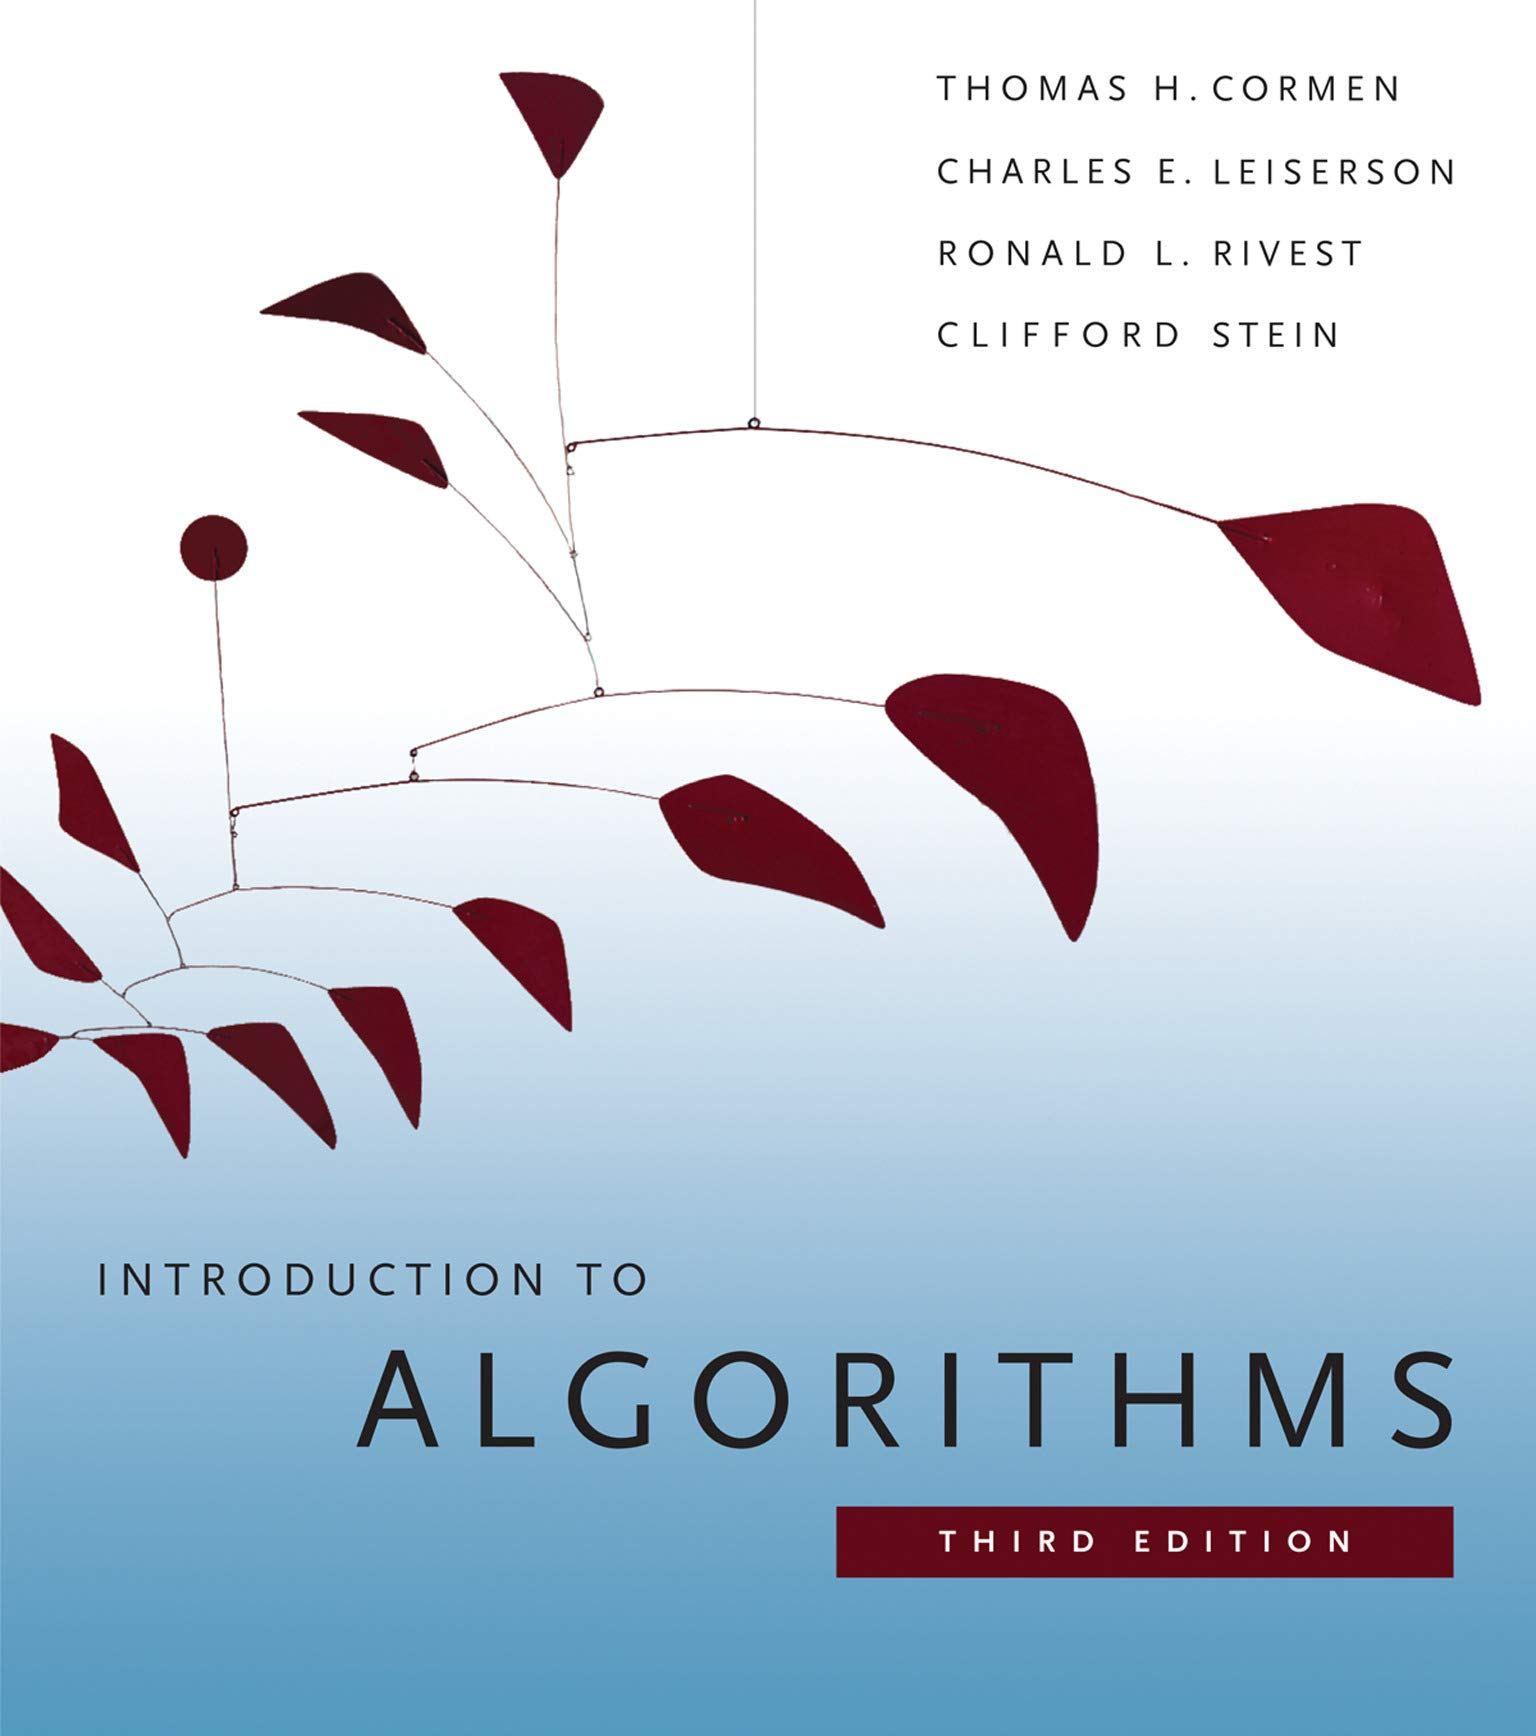
\includegraphics[scale=0.2]{./img/cormen.jpg}
      \caption{Cormen}
    \end{figure}

    \begin{minipage}{0.9\textwidth}
      \begin{flushleft} \large
        SABIER Corentin et CHASSAGNOL Rémi\\
        année 2020-2021\\[2cm]
      \end{flushleft}
    \end{minipage}

    \begin{minipage}{0.9\textwidth}
      \begin{flushright} \large
        \emph{Professeur:} CHORFI Amina\\
      \end{flushright}
    \end{minipage}

    \textsc{24 octobre 2020}

  \end{center}
\end{titlepage}

\clearpage

\tableofcontents

\clearpage

\section{Algorithmiques directes}

\subsection{Gauss}

\subsection{Cholesky}

\subsubsection{Principe}

Le principe de cette méthode est de trouver une matrice $R$ telles que $A =
R^{T}R$ où $R$ est une matrice triangulaire supérieure et $R^{T}$ est la matrice
transposée de R. Le système $Ax = b$ peut donc se diviser en deux sous-systèmes
$R^{T}y = b$ et $Rx = y$. Cette méthode est légèrement plus rapide que celle de
Gauss avec une complexité de $\frac{n^{3}}{3}$ au lieu de $\frac{2n^{3}}{3}$,
cependant elle nécessite que la matrice soit définie positive.

\subsubsection{L'Algorithme}

L'algorithme qui permet de trouver la matrice $R$ est le suivant:

\begin{lstlisting}
  Pour $i$ allant de $1$ a $n$:
      $s = a_{ii} - \sum_{j=1}^{i-1}r_{ji}^{2}$
      Si $s \leqslant 0$ alors:
          arret("la matrice n'est pas definie positive")
      Sinon
         $r_{ii} = \sqrt{s}$
         Pour $j$ allant de $i+1$ a $n$:
            $r_{ij} = \frac{a_{ij} - \sum_{k=1}^{i-1}}{r_{ii}}$
\end{lstlisting}

Ensuite il suffit de résoudre les deux sous-systèmes ce qui ce fait facilement
car la matrice est triangulaire.

\subsubsection{Les Variables}

Dans la fonction \textit{main} on initialise un matrice de taille
\textbf{LEN} qui est une constante pré-processeur. Les valeurs dans la matrice
dépendent de la constante \textbf{EXAMPLE} qui permet de déterminer
l’initialisation de la matrice via une fonction qui se situe dans le fichier
\textit{matrix.c}. Il y a en tout 8 matrices de testes qui sont celle demandé
dans la fiche de TP (chaque fonction remplit le tableau en fonction
de la définition de la matrice).

\begin{lstlisting}
  float *solus = malloc(LEN * sizeof(float));
  if (solus == NULL)
    exit(EXIT_FAILURE);
  float *b = malloc(LEN * sizeof(float));
  if (b == NULL)
    exit(EXIT_FAILURE);
  for (i = 0; i < LEN; i++) {
    b[i] = 1;
  }
  float **matrix = create_mat(LEN);
  mat(matrix, LEN, EXAMPLE);
  show(matrix, LEN);
  solver_cholesky(matrix, solus, b, LEN);
\end{lstlisting}

\subsubsection{Calcule de la matrice R}

Ensuite on calcule la matrice $R$ (le tableau à deux dimensions \textit{r}) à
l'aide de la fonction nommée \textbf{make\_R} qui suit l'algorithme ci-dessus. A
noter que cette fonction renvoi une erreur si la matrice en entrée n'est pas
définie positive ce qui stop le programme car le système n'est pas résolvable
avec cette méthode (en fait si la matrice n'est pas définie positive, la matrice
$R$ n'existe pas).

\begin{lstlisting}
void make_R(float **matrix, float **r, int n) {
  int i, j, k;   // loop var
  float sum = 0; // Used to calculate the sum of r_ki*r_kj
  float s;
  for (i = 0; i < n; i++) {
    s = matrix[i][i];
    for (j = 0; j < i; j++) {
      s -= r[j][i] * r[j][i];
    }
    if (s <= 0) {
      printf("La matrice n'est pas définie positive\n");
      exit(EXIT_FAILURE);
    } else {
      r[i][i] = sqrtf(s);
      for (j = (i + 1); j < n; j++) {
        sum = 0;
        for (k = 0; k < i; k++) {
          sum += r[k][i] * r[k][j];
        }
        r[i][j] = (matrix[i][j] - sum) / r[i][i];
      }
    }
  }
}
\end{lstlisting}

\subsubsection{Résolution des sous-systèmes}

Enfin la fonction \textbf{solver\_cholesky} résout les deux sous-systèmes de la
même manière qu'avec \textit{Gauss} sauf que les $a_{ii}$ ne sont pas forcement
égaux à 1 d'où la division pas $a_{ii}$. De plus, dans le premier sous-système,
la matrice $R^{T}$ est triangulaire inférieure, la résolution se fait donc en
commencent par calculer la valeur de la première inconnue.

\begin{lstlisting}
void solver_cholesky(float **matrix, float *solus_x, float *b, int n) {
  int i, j;
  float tmp;
  float *solus_y = malloc(n * sizeof(float));
  /*Creation of the matrix  R:*/
  float **r = create_mat(n);
  mat_0(r, n);
  make_R(matrix, r, n);
  /*Resolution de R^T * y = b*/
  transpose(r, n);
  for (i = 0; i < n; i++) {
    tmp = b[i];
    for (j = 0; j < i; j++) {
      tmp -= solus_y[j] * r[i][j];
    }
    solus_y[i] = tmp / r[i][i];
  }
  /*Resolution R * x = y*/
  transpose(r, n);
  for (i = (n - 1); i >= 0; i--) {
    for (j = (n - 1); j > i; j--) {
      solus_y[i] -= solus_x[j] * r[i][j];
    }
    solus_x[i] = solus_y[i] / r[i][i];
  }
  /*FREE*/
  free(solus_y);
  for (i = 0; i < n; i++) {
    free(r[i]);
  }
  free(r);
}
\end{lstlisting}

Cette fonction fait appelle à plusieurs autres fonctions:

\begin{itemize}
\item \textbf{create\_mat} qui retourne un tableau à deux dimensions de taille n
\item \textbf{mat\_0} qui remplit un tableau à deux dimensions de 0
\item \textbf{make\_R} vue ci dessus
\item \textbf{transpose} qui transpose la matrice qui lui est donnée en argument
\end{itemize}

Observons plus en détail la résolution du premier sous-système:

\begin{lstlisting}
  for (i = 0; i < n; i++) {
    for (j = 0; j < i; j++) {
      b[i] -= solus_y[j] * r[i][j];
    }
    solus_y[i] = b[i] / r[i][i];
  }
\end{lstlisting}

Voici la matrice r (après avoir été transposé):\\

\begin{vmatrix}
  a_{11} & 0 & \cdots & \cdots & 0\\
  a_{21} & a_{22} & 0 & \cdots & 0\\
  \vdots & \cdots & \ddots & 0 & 0\\
  a_{n1} & \cdots & \cdots & \cdots & a_{nn}\\
\end{vmatrix}\\

Nous résolvons $Ry = b$ donc:

\[y_{i} = \frac{b_{i} - \sum_{j=1}^{i}}{a_{ii}}\]

Ce qui se fait à l'aide des deux boucles ci-dessus.

A noter que ce programme alloue plus de mémoire que le précédent à cause de
l'utilisation du tableau \textbf{r} ce qui pourrait être problématique si on
travail avec des matrices de grandes taille.

\subsubsection{Les Tests}

\begin{itemize}
\item Bord \\
  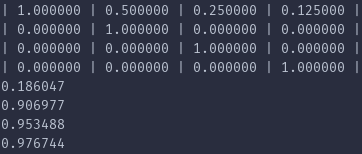
\includegraphics[scale=0.5]{./img/cholesky/bord.png} \\
  Cette solution est très imprécise avec cette méthode ce qui est du au fait que
  le programme crée la matrice $R$ et résous les deux sous-systèmes avec une
  matrice qui est déjà triangulaire supérieure ce qui génère une suite
  d'imprécisions dans les calcule. la vrai solution est:
  $x_{1} = \frac{1}{8} = 0.125 , x_{2} = 1 , x_{3} = 1 , x_{4} = 1$
\item Ding Dong \\
  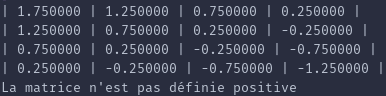
\includegraphics[scale=0.5]{./img/cholesky/ding_dong.png} \\
  Les programme retourne une erreur, en effet, la matrice n'est pas définie
  positive donc la méthode ne converge pas.
\item Franc \\
  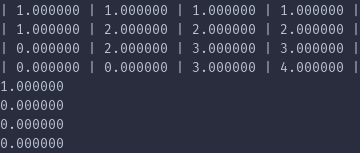
\includegraphics[scale=0.5]{./img/cholesky/franc.png} \\
  Le programme trouve la bonne solution.
\end{itemize}

\subsection{Conclusion sur les méthodes de résolution directes}

\textbf{j'aime les chats!!!}

\section{algorithmes itératifs}

Les algorithmes itératifs sont des algorithmes qui vont trouver une solution de
plus en plus précise à chaque itération. Ils partent d'un point de départ
arbitraire (un vecteur arbitraire) et vont converger vers la solution du
système.

\subsection{Jacobi}

\subsubsection{Principe}

Cet algorithme détermine les solutions du système $Ax = b$ en utilisant la
formule suivante:

\[x_{i}^{(k+1)} = \frac{b_{i} - \sum_{j=1}^{i-1}a_{ij}x_{j}^{(k)} -
  \sum_{j=i+1}^{n}a_{ij}x_{j}^{(k)}}{a_{ii}}\]

A chaque tours de boucle, l'algorithme calcule le nouveau vecteur $x^{(k+1)}$ en
utilisant la solution $x^{(k)}$ qu'il a calculé à l'itération précédente qui au
premier tour est un vecteur choisit arbitrairement qui sert de point de
départ. L'algorithme s'arrête quand la solution trouvée est convenable
$\parallel x^{(k+1)} - x^{(k)} \parallel \leqslant \varepsilon$ (ou
$\varepsilon$ est la précision choisit) ou quand il a fait un nombre de tours
pré-déterminer (pour éviter les boucles infinie si la méthode ne converge pas).

\subsubsection{L'algorithme}

\begin{lstlisting}
  Tant que $\varepsilon^{(k)} \geqslant \varepsilon$:
      $x_{i}^{(k+1)} = \frac{b_{i} - \sum_{j=1}^{i-1}a_{ij}x_{j}^{(k)} -
    \sum_{j=i+1}^{n}a_{ij}x_{j}^{(k)}}{a_{ii}}$
      $\varepsilon^{(k+1)} = \parallel x^{(k+1)} - x^{(k)} \parallel$
\end{lstlisting}

\subsubsection{Implémentation en C}

Les variables sont initialisées de la même façon que dans les méthodes directes
vues précédemment et le point de départ est \textbf{solus\_k} qui vaut $(1,
\dots, 1)$. La fonction qui calcule les solutions est la suivante:

\begin{lstlisting}
void jacobi(float **matrix, float *b, float *solus_k, int n) {
  int i, j;
  int compt = 0;
  int bool = 1;
  float *solus_k1 = malloc(n * sizeof(float));
  while (bool && compt < MAX) {
    for (i = 0; i < n; i++) {
      solus_k1[i] = b[i];
      for (j = 0; j < n; j++) {
        if (j != i)
          solus_k1[i] -= matrix[i][j] * solus_k[j];
      }
      solus_k1[i] /= matrix[i][i];
    }
    bool = test(solus_k1, solus_k, n);
    for (i = 0; i < n; i++) {
      solus_k[i] = solus_k1[i];
    }
    compt++;
  }
  printf("Nb tours: %d\n", compt);
  // FREE
  free(solus_k1);
}
\end{lstlisting}

Cette fonction utilise le même principe que l'algorithme ci dessus, elle
fait appel à une fonction \textit{test} qui retourne $\parallel x^{(k+1)} -
x^{(k)} \parallel \leqslant \varepsilon$ qui détermine l'arrêt (où sinon la
fonction s'arrête d'itérer à un nombre de tours maximum). A la fin =, on affiche
le nombre de tours effectués pour avoir un idée de la vitesse de convergence.

\subsection{Gauss-seidel}

\subsubsection{Le principe}

Cette méthode repose sur un principe similaire à celle de \textit{Jacobi},
cependant, elle utilises les solutions $x^{(k+1)}$ au fur et à mesure qu'elle
les calcules, ce qui lui permet de converger plus vite et donc de trouver une
solution plus rapidement. La formule utilisée par la méthode est la suivante:

\[x_{i}^{(k+1)} = \frac{b_{i} - \sum_{j=1}^{i-1}a_{ij}x_{j}^{\textbf{(k+1)}} -
  \sum_{j=i+1}^{n}a_{ij}x_{j}^{(k)}}{a_{ii}}\]

Cette méthode converge lorsque la matrice est définie positive et symétrique, ou
si elle est à diagonale dominante.

\subsubsection{L'algorithme}

L'algorithme est le même qu'avec \textbf{Jacobi} sauf qu'il utilise la nouvelle formule:

\begin{lstlisting}
  Tant que $\varepsilon^{(k)} \geqslant \varepsilon$:
      $x_{i}^{(k+1)} = \frac{b_{i} - \sum_{j=1}^{i-1}a_{ij}x_{j}^{\textbf{(k+1)}} -
    \sum_{j=i+1}^{n}a_{ij}x_{j}^{(k)}}{a_{ii}}$
      $\varepsilon^{(k+1)} = \parallel x^{(k+1)} - x^{(k)} \parallel$
\end{lstlisting}

\subsubsection{Le programme en C}

la fonction utilisée dans ce programme est très similaire à celle utilisée avec
\textbf{Jacobi} mis à part qu'elle utilise l'autre formule ce qui ce traduit
part un changement de variable.

\begin{lstlisting}
void gauss_seidel(float **matrix, float *b, float *solus_k, int n) {
  int i, j;
  int compt = 0;
  int bool = 1;
  float *solus_k1 = malloc(n * sizeof(float));
  while (bool && compt < MAX) {
    for (i = 0; i < n; i++) {
      solus_k1[i] = b[i];
      for (j = 0; j < i; j++) {
        solus_k1[i] -= matrix[i][j] * solus_k1[j];
      }
      for (j = i+1; j < n; j++) {
	solus_k1[i] -= matrix[i][j] * solus_k[j];
      }
      solus_k1[i] /= matrix[i][i];
    }
    bool = test(solus_k1, solus_k, n);
    for (i = 0; i < n; i++) {
      solus_k[i] = solus_k1[i];
    }
    compt++;
  }
  printf("Nb tours: %d\n", compt);
  // FREE
  free(solus_k1);
}
\end{lstlisting}

La modification est au niveau de la ligne \textbf{10}, on utilise $x^{(K+1)}$ au
lieu de $x^{(k)}$

\subsection{Comparaison des résultats}

\subsubsection{Matrice symétrique à diagonale dominante}

Dans cette exemple nous allons résoudre deux systèmes avec la même matrice
symétrique à diagonale supérieure:

Résolution de:

\[
\begin{pmatrix}
  4 & 1 & 1 & 0\\
  1 & 4 & 0 & 1\\
  1 & 0 & 4 & 1\\
  0 & 1 & 1 & 4\\
\end{pmatrix} X =
\begin{pmatrix}
  15\\
  15\\
  19\\
  11\\
\end{pmatrix}
\]

Voici la solution trouvée par \textbf{jacobi}:

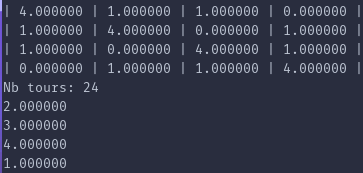
\includegraphics[scale=0.5]{./img/jacobi/jac_ex_1.png}

Voici la solution trouvée par \textbf{gauss seidel}:

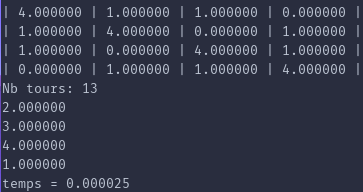
\includegraphics[scale=0.5]{./img/gauss_seidel/g_e_ex_1.png}

On constate que la solution trouvée avec les deux méthodes et la même et si on
regarde le nombre de tours effectués, on voit que \textbf{gauss-seidel} converge
presque deux fois plus vite que \textbf{jacobi}.

Résolvons le même système en faisant varier les valeurs dans b de $+0.005$:

Voici la solution trouvée par \textbf{jacobi}:

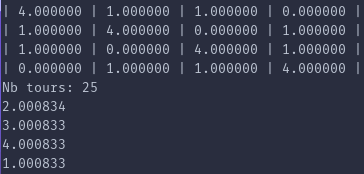
\includegraphics[scale=0.5]{./img/jacobi/jac_ex_1_mod.png}

Voici la solution trouvée par \textbf{gauss seidel}:

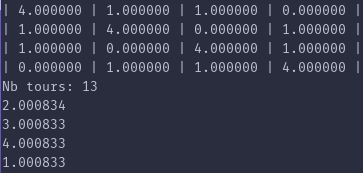
\includegraphics[scale=0.5]{./img/gauss_seidel/g_e_ex_1_mod.png}

On constate que les résultats n'ont pas beaucoup variés, donc la modification
effectuée sur b sont bien gérées par le programme donc les méthodes sont stables.

\subsubsection{Une Erreur}

Avec ce test, on voit que si la matrice ne respecte pas les contrainte requises
par les méthodes, celle-ci tournes à l'infini sans jamais converger vers la
solution du système (le programme s'arrête car la fonction est limité à 100 tours).

Résolution de:

\[
\begin{pmatrix}
  1 & 2 & 1\\
  2 & 2 & 3\\
  5 & 1 & 8\\
\end{pmatrix} X =
\begin{pmatrix}
  2\\
  -1\\
  3\\
\end{pmatrix}
\]

Voici la solution trouvée par \textbf{jacobi}:

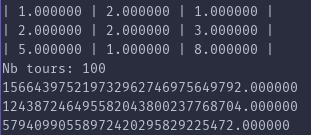
\includegraphics[scale=0.5]{./img/jacobi/jac_ex_3.png}

Voici la solution trouvée par \textbf{gauss seidel}:

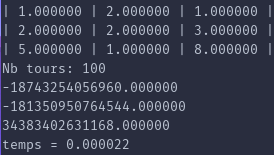
\includegraphics[scale=0.5]{./img/gauss_seidel/g_e_fail.png}

\clearpage

%=============================================
%---------------annexes pour code-------------
%=============================================

\begin{appendix}
  \section*{Gauss}

  \begin{lstlisting}

  \end{lstlisting}
\end{appendix}
\clearpage

%=============================================

\begin{appendix}
  \section*{Cholesky}
  \lstinputlisting{./prog/cholesky.c}
\end{appendix}
\clearpage

%=============================================

\begin{appendix}
  \section*{Jacobi}
  \lstinputlisting{./prog/jacobi.c}
\end{appendix}
\clearpage

%=============================================

\begin{appendix}
  \section*{Gauss Seidel}
    \lstinputlisting{./prog/gauss_seidel.c}
\end{appendix}

\end{document}
